\section{Tests and results}
\subsection{Dataset}
The dataset used is the SpamAssassin Public Corpus provided by SpamAssassin at \url{http://spamassassin.apache.org/publiccorpus/}, freely available for development purposes (maintainers warn to not use the dataset for training a live system). It contains about 6400 mails in english language, collected from 2002 to 2005, with approximately the 31\% of the mails being spam.

\subsection{Modalities}

\subsection{Features of spam and ham mails}
\label{featuresused} The following features have been selected as relevant and are tracked by the network:
\begin{itemize}[noitemsep]
  \item the number of words written in uppercase characters: since it is considered the equivalent of screaming, many spammers use this gross trick to gain attention;
  \item the number of urls found: we expect to find a lot of addresses of websites where to buy goods or where some criminal activity will be performed (phishing, stealing credentials, etc.);
  \item the number of email addresses: for the same reason of the previous feature. Furthermore, spammers operate on a large scale, so it is possible for a spam mail to have multiple recipients;
  \item the number of words shorter than a given threshold (given as a parameter): a trick to fool a system based on word classification is to hide the words. One of the most common and easier way of accomplish this, is to separate each letter with spaces. Since our token separation relies on whitespaces between words, a word like \texttt{s\textvisiblespace p\textvisiblespace a\textvisiblespace m} (with spaces between characters), which a human will easily understand as a single one, will be classified by the network as four different words. In a common, correct plain english text, the ratio of short words like \verb!a! or \verb!I! will be substantially lower, not to mention other random letters;
  \item the number of non-address words longer than a given threshold (parameter): similarly to the previous feature, a spam mail is likely to contain a number of very long, meaningless words much higher than a ham mail. Since there aren't many very long legit words\footnote{The average length of english words is slightly higher than 5 (\url{http://www.puchu.net/doc/Average_Word_Length}), while the majority of words appearing in a text is from 2 to 5 letters long. \citep{STUL:STUL109}}, this is a reasonable feature to track;
  \item the number of words in the form \verb!username@host!: the tests have shown that the ham mails in the SpamAssassin Public Corpus contain many tokens of this type;
  \item the number of words in ``title'' format (first letter capital, remaining letter lowercase);
  \item the number of words in a mail.
\end{itemize}

Many other interesting features can also be used: for example, a heavy use of images as text replacement, the consistency of the email header, the consistency of the urls with the link they claim to go, the list of people the user have mailed before, the provenance of the mail from a known spammer or IP range, the correctness of words (by checking a dictionary), to name a few. All of these features require a semantic analysis of the mail, which goes beyond the purpose of this project, since no one of these features is directly connected to Bayesian networks. Nonetheless, all of these features can be used by a Bayesian network, just like the previous ones, and are very likely to increase the accuracy of the classification.

It should be noted that while some of these features are common for the majority of spam, some others are derived from our particular mail archive. Moreover, since many of the mails in the archive are ten years old, more recent spam mails may contain different features.% The maintainers of the archive warn to use the archive only for development purposes, not in a live system.

\subsection{The design parameters}
The Bayesian network requires some parameters to be tuned: for example, the ``spamicity'' threshold (how much the normalized probability of being spam should be to be really considered as spam), or the ``weight'' of the feature stats with respect to the word stats when computing the final probability. Different parameter configurations lead to obtain different accuracy values, so we have to choose the best one.

We'll now present the results obtained. Since there are multiple degrees of freedom, we show how the accuracy varies when trying to change one single parameter at time, all the other ones being set to their optimal value. Because of the random choice of the emails used for training, validation and testing, multiple tests have been performed, and the results in the following paragraphs are the medians of the values observed.

\paragraph{Size of the training and validation sets}
For finding the best size of the training set, we have begun with few mails, then we have tried to increase the size of the training set until the accuracy has started to decrease (the \textit{early stopping} technique). The size of the validation set is a quarter of the size of the training set. Each value in table \ref{tab:sizebags} is intended to be doubled, being the number of mails for each class to be used.

\begin{center}
\begin{table}[h]
\begin{minipage}{.5\linewidth}
\begin{tabular}{cccc}
\toprule
\multicolumn{2}{c}{Size of sets} \\
\cmidrule(r){1-2}
Training & Validation & \shortstack{Validation\\ accuracy} & \shortstack{Testing\\ accuracy}\\
\midrule
50   & 12     & 0.5416667 & 0.739\\
100  & 25     & 0.78 & 0.7725 \\
200  & 50     & 0.72 & 0.7935 \\
500  & 125    & 0.788 & 0.842 \\
800  & 200    & 0.71 & 0.8515 \\
1000 & 250    & 0.73 & 0.849 \\
\bottomrule
\end{tabular}
\end{minipage}
\begin{minipage}{.5\linewidth}
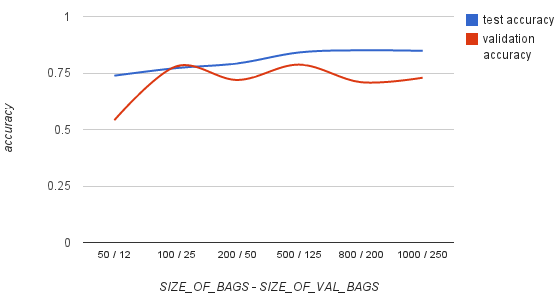
\includegraphics[width=1\textwidth]{img/tests/size_bags.png}
    \label{fig:sizebags}
\end{minipage}
\caption{Accuracy with varying size for training set and validation set.}
\label{tab:sizebags}
\end{table}
\end{center}

As we see, the best accuracy is obtained using 800 spam mails and 800 ham mails for training, and 200+200 mails for validation. Furthermore, if we compare all the results, we observe that with fewer mails the variance of the results is higher.

\paragraph{Size of test sets}
As for training and validation set, we look for the optimal size of the test set. Because of the self-improving nature of Naive Bayes networks, we expect the accuracy to grow along with the size of the test set. Results of the trials are shown in table \ref{tab:sizetest}.

\begin{center}
\begin{table}[h]
\begin{minipage}{.5\linewidth}
\begin{tabular}{cccc}
\toprule
Size of test set & \shortstack{Validation\\ accuracy} & \shortstack{Testing\\ accuracy}\\
\midrule
100  & 0.71 & 0.82     \\
200  & 0.71   & 0.835    \\
500  & 0.71 & 0.827    \\
800  & 0.71 & 0.842605 \\
1000 & 0.71   & 0.8515   \\
\bottomrule
\end{tabular}
\end{minipage}
\begin{minipage}{.5\linewidth}
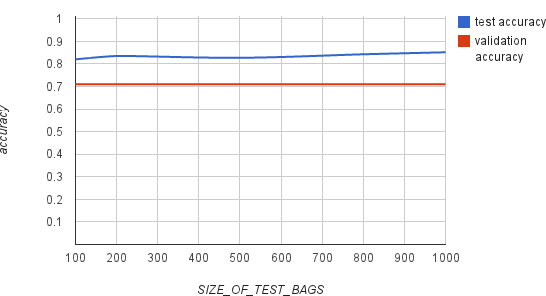
\includegraphics[width=1\textwidth]{img/tests/size_test.png}
    \label{fig:sizetest}
\end{minipage}
\caption{Accuracy with varying size of test sets.}
\end{table}
\label{tab:sizetest}
\end{center}

As expected, the more mails are processed, the higher accuracy we get. We stopped at 1000+1000 mails, because it takes a long time to process all the mails, and because the increment of accuracy begins to slow down.

\paragraph{``Spamicity'' threshold}
\label{spamthrtest} Another very important parameter is what is sometimes called the ``spamicity'' threshold, namely the value that the normalized probability $\frac{p_{spam}}{p_{spam} + p_{ham}}$ must reach for the mail to be classified as spam. This is crucial: a low threshold will bring in many false positives (good mails will be marked as spam), while a too high threshold will classify some spam mails as ham, thus having a lot of false negatives. Anyway, the choice of the threshold to be $0.5$ may not be obvious, since we may want to be more tolerant with words we have never met before, or we may consider the chance of false positive too bad for us, and therefore lift the threshold to ensure this fact, allowing at the same time some spam to pass through the filter. More importantly, we desire a similar number for false positives and false negatives, since this is an index of well-balanced classification. For this reason, this value is only the starting value of the threshold, which will be tuned by the classifier according to the number of misclassified items. Furthermore, given the nature of bayesian networks, a fair threshold guarantees that the classifier remains stable, meaning that it will continue guessing with the same ham and spam ratio, while a very unbalanced number of misclassifications will make the classifier leaning towards too many guesses of a single kind (the more mails are misclassified as spam, the more words will erroneously contribute to spam in future classifications, same for ham).

\begin{center}
\begin{table}[h]
\begin{minipage}{.5\linewidth}
\begin{tabular}{cccc}
\toprule
Threshold & \shortstack{Validation\\ accuracy} & \shortstack{Testing\\ accuracy}\\
\midrule
0.1  & 0.725 & 0.834\\
0.2  & 0.71 & 0.8515 \\
0.3  & 0.77 & 0.8305 \\
0.4  & 0.7 & 0.8595 \\
0.5  & 0.72 & 0.8455 \\
0.6  & 0.7125 & 0.841 \\
0.7  & 0.74 & 0.839 \\
0.8  & 0.7 & 0.848 \\
0.9  & 0.705 & 0.8305 \\
\bottomrule
\end{tabular}
\end{minipage}
\begin{minipage}{.5\linewidth}
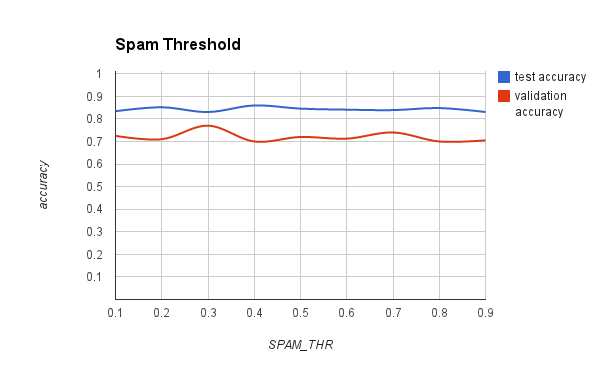
\includegraphics[width=1\textwidth]{img/tests/spam_thr.png}
    \label{fig:spamthr}
\end{minipage}
\caption{Accuracy with varying ``spamicity'' threshold.}
\end{table}
\label{tab:spamthr}
\end{center}

We see that the accuracy is similar for all the starting values. Anyway, when looking at the final value that the threshold take, we see that most of the times it lies around 0.2, so this is our default value. The other starting values get a similar accuracy because when having multiple errors in the beginning, the threshold changes rather quickly.

\paragraph{Relevance threshold}
As we have already discussed in section \ref{notesonimpl}, we provide a customizable threshold to exclude from computation the words and the features that give little contribution to the final probabilities. In table \ref{tab:relevance} we see what is the most convenient value.

\begin{center}
\begin{table}[h]
\begin{minipage}{.5\linewidth}
\begin{tabular}{ccc}
\toprule
Threshold & \shortstack{Validation\\ accuracy} & \shortstack{Testing\\ accuracy}\\
\midrule
0.15  & 0.6925 & 0.703  \\
0.2   & 0.6925 & 0.8025 \\
0.25  & 0.71 & 0.8515   \\
0.3   & 0.605 & 0.798   \\
0.35  & 0.71 & 0.6665   \\
\bottomrule
\end{tabular}
\end{minipage}
\begin{minipage}{.5\linewidth}
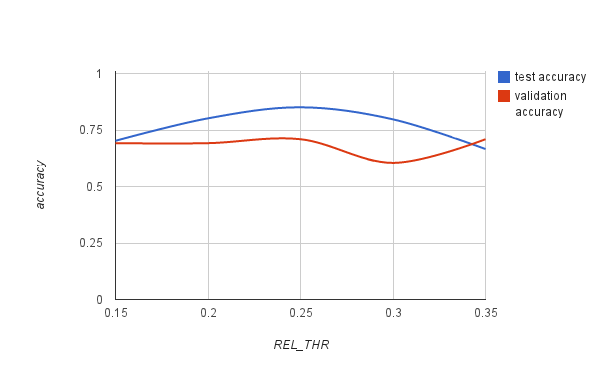
\includegraphics[width=1\textwidth]{img/tests/rel_threshold.png}
    \label{fig:relthreshold}
\end{minipage}
\caption{Accuracies obtained when varying the relevance threshold.}
\end{table}
\label{tab:relevance}
\end{center}

\paragraph{Feature/words stats proportion}
Another problem is to determine how much weight should we assign to the features statistics, and how much to the word statistics.

The final formula for spam is $p_{spam} = W \times p_{fs} + (1-W) \times p_{ws}$, where $p_{spam}$ is the probability of the mail being spam (yet to be normalized), $p_{fs}$ is the probability of being spam computed using the statistics of the features, $p_{ws}$ is the probability of being spam computed using the statistics of the words, and $W$ is the parameter we want to adjust. The formula for ham is the dual.

A value close to $1$ will lead to a classification based solely on the features, thus almost ignoring the actual content of the mail. A low value will instead disregard the features, and therefore many useful and common characteristics of spam mails.

\begin{center}
\begin{table}[h]%[!htb]
\begin{minipage}{.5\linewidth}
%\begin{scriptsize}
\begin{center}
\begin{tabular}{ccccc}
\toprule
Threshold & \shortstack{Validation\\ accuracy} & \shortstack{Testing\\ accuracy} \\
\midrule
0.0001 & 0.7025 & 0.8595 \\
0.001  & 0.7125 & 0.8275 \\
0.01   & 0.6925 & 0.832  \\
0.1    & 0.6725 & 0.801  \\
0.2    & 0.745  & 0.7945 \\
0.4    & 0.7325 & 0.7795 \\
0.6    & 0.6925 & 0.739  \\
0.8    & 0.73   & 0.7115 \\
\bottomrule
\end{tabular}
\end{center}
%\end{scriptsize}
\end{minipage}
\begin{minipage}{.5\linewidth}
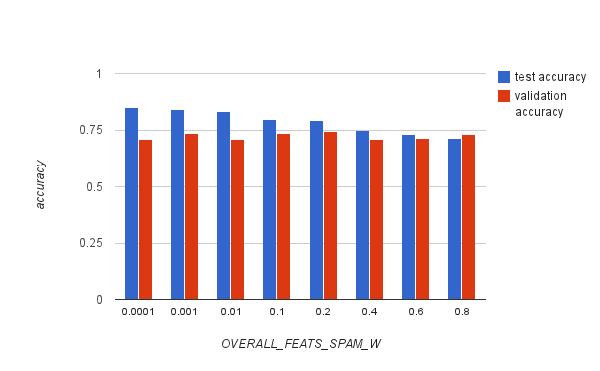
\includegraphics[width=1\textwidth]{img/tests/feats_threshold_1.png}
    \label{fig:featuresthreshold}
\end{minipage}
\caption{Validation and final accuracies, with varying feature statistics thresholds.}
\label{tab:featsthr}
\end{table}
\end{center}

We clearly see (table \ref{tab:featsthr}) that the more the threshold approaches zero, the better results it yields. This means that, at least with the dataset we are using, a classifier based only on words works better than a classifier which accounts also the general features of the mail. It is interesting to note that the validation accuracy remains almost at the same level, while the real difference comes out during the testing step, when a much higher number of mails are processed, and the network can thus learn much more. 

\subsection{Analysis of results}
Here we show and analyze some interesting results observed. Of course, these statistics apply only for the SpamAssassin dataset, and may not be generalized.
% \begin{center}
% \begin{tabular}{lcc}
% \toprule
% & \multicolumn{2}{c}{Occurrences} \\
% \cmidrule(r){2-3}
% Feature & \# in spam & \# in ham \\
% \midrule
% \# of all-caps words                            & 10    & 0.1 \\
% \# of alphanumerical words                      & 20    & 0.2 \\
% \# of string in user/hosts form                 & 50    & 0.3 \\
% \# of links                                     & 100   & 0.4 \\
% \# of mail addresses                            & 10    & 0.1 \\
% \# of all lowercase words                       & 20    & 0.2 \\
% \# of words with only the first letter capital  & 50    & 0.3 \\
% \# of ``short words''                           & 10    & 0.0 \\
% \# of non-address ``very long'' words           & 100   & 0.4 \\
% \# of non-valid words                           & 50    & 0.3 \\
% \# of numbers                                   & 100   & 0.4 \\
% \bottomrule
% \end{tabular}
% \end{center}

As expected, ``very short'' and ``very long'' words (out of our thresholds) are mostly common in spam mails, as well as all-caps words, non-valid words and mail addresses. Spam mails also contain an average number of words higher than ham ones. Surprisingly, in the SpamAssassin dataset ham mails contain more links than spam mails.

%\paragraph{Most common words}
It's interesting also to look at the statistics of the single words. We have already discussed about how the distribution of unusually long words. In our dataset, the words that contribute most to ham are technology-related words like \texttt{debian}, \texttt{cpp}, \texttt{gaim}, 0\texttt{xdeadbeef} (hex code used by \textsc{ibm}). Spam mails, instead, are characterized by meaningless words and words that suggest the selling of some goods, in particular drugs, as, for example, \texttt{botanical}, \texttt{dieting}, \texttt{aphrodisia}.

% \begin{center}
% \begin{tabular}{cc}
% \toprule
% Words in spam & Words in ham \\
% \midrule
% \# of all-caps words                            & matthias \\
% \# of alphanumerical words                      & 0xdeadbeef \\
% \# of string in user/hosts form                 & gaim \\
% \# of links                                     &  \\
% \# of mail addresses                            & 10 \\
% \# of all lowercase words                       & 20 \\
% \# of words with only the first letter capital  & 50 \\
% \# of ``short words''                           & 10 \\
% \# of non-address ``very long'' words           & 10 \\
% \# of non-valid words                           & 50 \\
% \# of numbers                                   & 10 \\
% \bottomrule
% \end{tabular}
% \label{tab:commonwords}
% \end{center}
